\documentclass[a4paper,11pt]{article}
\usepackage[left=2cm,text={17cm,24cm},top=3cm]{geometry}

\usepackage{times}
\usepackage[czech]{babel}
\usepackage[utf8]{inputenc}
\usepackage[unicode]{hyperref}
\newcommand{\czuv}[1]{\quotedblbase #1\textquotedblleft}
\usepackage{graphicx}
\usepackage{caption}
\usepackage{pdflscape}
\usepackage{graphicx}

\makeatletter

\renewcommand\@pnumwidth{1.5em}   
\newcommand\My@secwidth{2.5ex}   
\newcommand\My@subsecwidth{4.5ex} 


\newcommand{\My@dotfill}{\leavevmode\xleaders\hbox to 1.5mm{\hfil.}\hfill}



\renewcommand*\l@subsection[2]{%
	\ifnum \c@tocdepth>1
		\setlength\@tempdima{\My@subsecwidth}%
		\setlength\@tempdimb{\My@secwidth}%
		\begingroup
			\parindent \z@ \rightskip \@pnumwidth
			\parfillskip -\@pnumwidth
			\leavevmode
			\advance\leftskip\@tempdima
			\advance\leftskip\@tempdimb
			\hskip -\leftskip
			\hskip \@tempdimb
			#1\nobreak\My@dotfill \nobreak\hb@xt@\@pnumwidth{\hss #2}\par
		\endgroup
	\fi}

\makeatother
%----------------------------------------------------------%
\begin{document}

\begin{titlepage}
    \begin{center}
        \Huge
        \textsc{Vysoké učení technické v~Brně\\
               \huge Fakulta informačních technologií}\\
               
        \vspace{\stretch{0.382}}
        \LARGE
                Mikroprocesorové a vestavěné systémy\\
                \Huge  Hodiny s budíkem na bázi modulu (RTC)\\
        \vspace{\stretch{0.618}}
    \end{center}
    
    {\Large \today \hfill
                Vladislav Mikheda\\
                }
\end{titlepage}

\newpage
\section{Úvod}
Cílem projektu bylo implementovat digitální hodiny s budíkem s využitím modelu \texttt{RTC} na platformě \texttt{FitKit3}.
\subsection{Motivace}
Jak už bylo popsáno, cílem je implementovat digitální hodiny s budíkem. K tomuto problému by se dalo přistupovat několika způsoby. 
\begin{itemize}
    \item Řešení pomocí elektrických(číslicové)systémů. Toto řešení by vypadalo jako připojení několika číslicových součástek k desce(čítač, dekodér atd.), realizace tohoto řešení by bylo dost velké, příliš nákladové na realizaci a odvedená práce by za výsledek nestála. 
    \item Dalším řešením je naprogramovat budík software, toto řešení má hodné výhod: jednoduchá a rychlá implementace. Je však problém, na kterém zařízení  tento program poběží.
    \item Třetí přistup a je ten který jsem v projektu použil, vestavěný systém (en. embedded system), který kombinuje software a hardware.
\end{itemize}
 Pro dosaženi cíle je vhodnější využit třetí přistup který má další výhody:
 \begin{enumerate}
     \item  Jednoduchost vývoje, jelikož samotný program je napsán softwarově .
     \item  Hardware na kterém je tento software spuštěn.
     \item  Hardwarové komponenty které jsou použité (RTC atd.) a velkou výhodou je že dá se přidat další různé komponenty (obrazovka pro zobrazení času, atd.).
 \end{enumerate}
\subsection{Použité nástroje}
Pro řešeni projektu bylo použito zařízení \texttt{FitKit3}, jako operační systém byl použit \texttt{Windows 11}, vývojové prostředí \texttt{Kinetis Design Studio 3.0.0 IDE} pomocí kterého je možné překládat zdrojový kód, nahrávat do \texttt{FitKit3} a opravovat program. Pro komunikace se zařízením přes \texttt{UART} byly využity \texttt{Putty}. 

\subsection{Dekompozice zadaní}
\label{sec:dek}
Před začátkem řešení projektu byla provedena dekompozice problému:
\begin{itemize}
    \item Konfigurace zařízeni.
    \item Nastavení času.
    \item Konfigurace budíku.
    \begin{itemize}
        \item Výběr zvukové signalizace.
        \item Výběr světelné signalizace.
        \item Nastavení opakování.
    \end{itemize}
    \item Nastavení času budíku.
    \item Realizace vypnutí a zapnutí budíku.
\end{itemize}
\subsection{Hardware}
K realizaci projektu byly použity následující hardwarové komponenty: RTC, UART, diody, tlačítka a bzučák.
\subsubsection{Obecná konfigurace MCU}
Na začátku bylo provedeno nastavení hodinového podsystému(\texttt{reg. MCG\_C4}), dal dělič byl nastaven na \\nulu(\texttt{reg. SIM\_CLKDIV1}), vypnut \texttt{watchdog}(\texttt{reg. WDOG\_STCTRLH}), pak zapnuty hodiny pro \texttt{UART}, \texttt{RTC}, port \texttt{B}, port \texttt{E}, port \texttt{A}. Pro zapínaní hodin byly využity masky a registry \texttt{SIM\_SCGC5,  SIM\_SCGC1,  SIM\_SCGC6}.
\subsubsection{UART}
Byl využit \texttt{UART5}. Pro konfigurace byly využity registry \texttt{ UART5\_C1, UART5\_BDH, UART5\_BDL, UART5\_C4,  UART5\_C3,  UART5\_MA1,  UART5\_MA2, UART5\_S2} a byla nastavena  přenosová rychlost \texttt{115200Bd}, přenos \texttt{8 bitu bez parity}.\\
Za běhu byly využity registry: \texttt{UART5\_S1} flagy \texttt{TDRE, TC} jsou využity pro sledovaní, zda je datový kanál zaneprázdněn, flag \texttt{RDRF}
je využity pro sledovaní je-li datový registr naplněn. Registr \texttt{UART5\_D} pro čtení a zápis dat.
\subsubsection{RTC}
Pro konfigurace byly využity registry: \texttt{RTC\_CR} flag \texttt{SWR} pro 
resetovaní všech \texttt{RTC} registrů, \texttt{OSCE}  pro zapnutí oscilátoru. \\
Za běhu byly využity registry: \texttt{RTC\_SR} bit \texttt{TCE} zapnuti a vypnuti čítače sekund. Registr \texttt{RTC\_TSR} pro nastavení a čtení času. Refistr \texttt{RTC\_TAR} pro nastavení a ctěni času budíku. Registr \texttt{RTC\_IER} flag \texttt{TAIE} pro zapnutí, vypnutí a přerušení budíku. 
\subsubsection{Porty}
Pro \texttt{UART5}, diody, tlačítka a bzučák byly nastaveny porty. Pro nastavení byl použit registr \texttt{PORTx\_PCRn} kde \texttt{x} je název portu a \texttt{n} je pin na který je připojen komponent. \\
U tlačítek byly nastaveny přerušení. Bzučák a diody za běhu programu se aktivují a deaktivují pomocí registru \texttt{GPIOx\_PDOR} pro tento registr byla využita maska \texttt{PTx\_PDOR}  kde \texttt{x} je název portu.

\subsection{Sowtware}
Pro účely projektu byla použita knihovna pro komunikaci s zařízením \texttt{MK60D10.h}. Pro práce s časem je použita knihovna \texttt{time} která umožní práce s Unix formátem času.
\section{Implementace}
Na začátku podle dekompozice která je uvedená v sekci \ref{sec:dek} byl navržen Konečný automat obrázek č:\ref{obrazek:1}. Pak byla provedena inicializace komponentů, při inicializaci kód byl inspirován příklady z laboratoře a příklady programů na \texttt{FitKit3} které byly zaznamenány na přednášce. Dál bylo implementováno řešení.
\subsection{Rozdělení}
Program byl rozdělen do jednotlivých souboru pro přehlednost. Každý soubor kromě \texttt{main.c} reprezentuje nějakou pomocnou část. 
\begin{itemize}
    \item init -- reprezentuje inicializaci komponentu a \texttt{MCU}.
    \item addons -- reprezentuje funkce blikání diod atd. 
    \item times -- reprezentuje funkci práce s časem.
    \item uart -- reprezentuje funkci práce s \texttt{UART}.
    \item main -- hlavní soubor
\end{itemize}
\begin{figure}[h]
\center{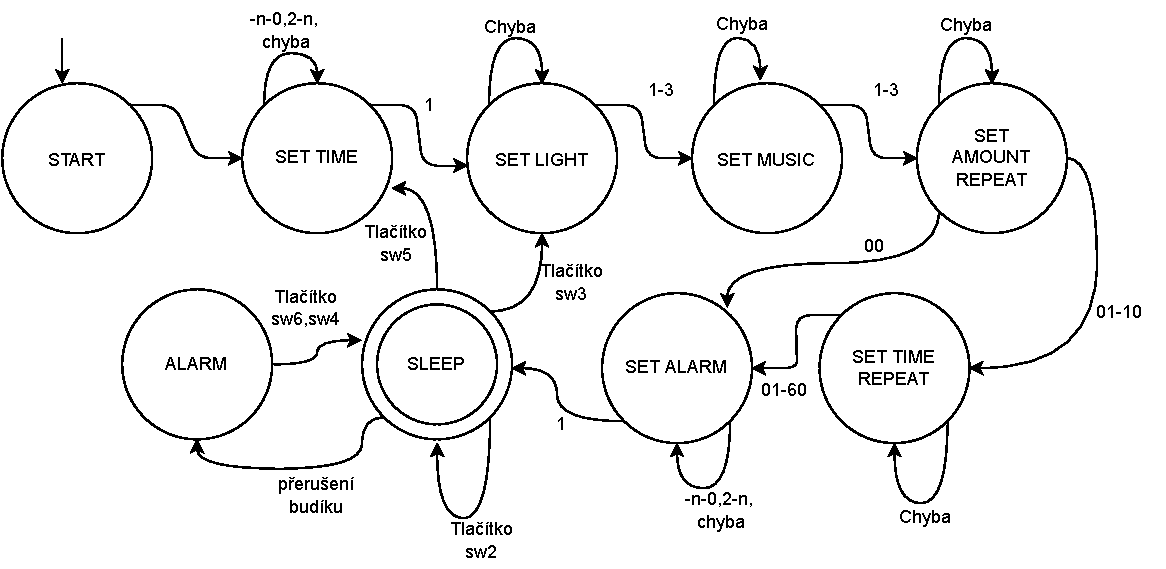
\includegraphics[scale=0.7]{img/automat.pdf}}
\caption{Konečný automat}
\label{obrazek:1}
\end{figure}
\subsection{Hlavní smyčka }
V hlavní smyčce programu je implementován konečný automat.\\
Po zapnutí zařízení je potřeba nastavit čas. Pak jsou dvě možnosti: přejít do režimu spánku nebo nastavit budík. Režim spánku je nekonečná smyčka ze které můžete vystoupit pomocí přerušení (stisknutím tlačítka). Při nastavování budíku bude uživatel muset nastavit: zvukovou a světelnou signalizaci, a poté zvolit, kolikrát lze budík opakovat. Pak nastavit čas probuzení. Budík poté přejde do režimu spánku.
\subsection{Práce s časem}
Pro práci s časem bylo rozhodnuto použít unixový čas, který ukazuje počet sekund od roku 1970. Toto řešení má problémy, které jsou popsány v sekci \ref{sec:prob}.
\subsubsection{Nastavení času}
Uživatel zadá čas ve formátu \czuv{dd-mm-YYYY HH:MM}. Pomocí funkce \texttt{strptime} bude tento čas převeden do struktury \texttt{tm} a  bude zkontrolována platnost dat, poté bude převeden na sekundy pomocí funkce \texttt{mktime} a zapsán do registru \texttt{RTC\_TSR}.
\subsubsection{Nastavení času buzení}
\label{sec:zapbuz}
Nastavení času budíku je podobné obecnému nastavení času. Uživatel zadá čas ve formátu \czuv{HH:MM}. Pak jsou dvě možnosti: buď bude budík nastaven na dnešek, pokud čas neuplynul, nebo na zítra. Porovnání času probíhá pomocí převodu času na zařízení do struktury \texttt{tm} a jeho porovnáním s nastaveným časem budíku.\\
Dále zkopírujeme aktuální čas na zařízení, a odečítáme tolik sekund, kolik je potřeba aby byl začátek dne(00:00) a pak se přidává počet sekund zbývajících do buzení, a nastavíme registr \texttt{RTC\_TAR}.

\subsection{Buzeni}
Pokud je budík zapnutý(je zapnuto přerušení budíku) když se čas ve dvou registrech \texttt{RTC\_TAR a RTC\_SRT} shoduje, bude vyvoláno přerušení . Kde flag přerušení bude vypnut a nastavěn stav konečného automatu který reprezentuje buzení. Buzení probíhá zvukovou a světelnou signalizací, dokud uživatel nevypne budík nebo nezapne opakovaní. Stav buzení lze změnit jenom přerušením.

\subsection{Zvukovou a světelnou signalizaci}
Zvukovou a světelnou signalizaci jsou implementovány v souboru \texttt{addons}. Poté, co uživatel vybere signalizaci, bude jeho volba uložena v globální proměnné. V režimu buzení budou signalizace vybírány pomocí \texttt{switch}.

\subsection{Přerušeni}
Přerušení může být zapnuté buď použitím tlačítek které jsou nastaveny nebo zapnutím buzení, je to popsáno v sekci \ref{sec:zapbuz}. 
\subsubsection{Tlačítko SW2}
Při stisknutí tlačítka sw2 na obrazovku bude vypsán aktuální čas zařízení a jestli budík je nastaven bude vypsán i čas buzení. Z registru \texttt{RTS\_TSR} bude zkopírován aktuální čas v sekundách a bude  převáděn pomocí funkce \texttt{localtime\_r} do struktury \texttt{tm} a pak už pomocí funkce \texttt{strftime} převeden do formátu řetězce.
\subsubsection{Tlačítko SW6}
Stisknutím tlačítka \texttt{sw6} lze odstranit všechny budíky nebo vypnout signalizaci budíku při buzení nebo když budík není nastaven, nastavit ho znovu na čas který už byl zadán uživatelem, nastavení je popsáno v sekci \ref{sec:zapbuz}.
\subsubsection{Tlačítko SW4}
 Při stisknutí tlačítka vypne se signalizace buzení a když je nastaven opakovaně nastaví se budík na novy čas který se počítá jako čas vypnutí budíku + čas za kolik minut budík musí znova zazvonit.\\
Při stisknutí tlačítka \texttt{sw4} přerušení bude vyvoláno ale pokud budík není ve stavu buzení nic se nestane.
\subsubsection{Tlačítko SW5}
Vyvolá se přerušení, hodiny a budík budou resetovány a vrátí se do začátečního stavu, konečný automat bude převeden do stavu nastavení času. Toto přerušení nebude obslouženo když budík ve stavu buzení.
\subsubsection{Tlačítko SW3}
Při stisknutí tlačítka sw3, automat přepne se do stavu nastavení budíku a úmožní uživatelům nastavit budík na nový čas.

\section{Shrnutí}
\subsection{Testovaní}
Testování proběhlo manuálně. Bylo provedeno několik testů. Postup provádění testovaní: na začátku je nutné nastavit aktuální čas, dál nastavit signalizace a opakování, pak nastavit budík.\\
Při různých testech nastavení signalizace a opakování bylo zvolené různě. Na začátku bylo testováno funguje-li buzení, dál bylo testováno opakování a vypínaní/zapínání budíku, poslední etapou testovaní je testovaní různé světové a zvukové signalizace. Z testovaní nahoře jde říct že projekt je úplně funkční.

\subsection{Problém unixového času}
\label{sec:prob}
Řešení s využitím unixového času má problém v tom že \texttt{RTC\_TSR} registr je 32 bitovy a když čas se počítá z 1970 roku tak v roce 2038 bude přetečení. Které způsobí nefunkčnost budíku. Ale v současné době neovlivni chování zařízení.

\end{document}
